\section{Ejemplos del lenguaje de marcado Latex}

Ejemplos de citas: el libro \textit{The \LaTeX\ Companion}
\cite{latexcompanion}, un paper de Einstein \cite{einstein}, dos informes técnicos de relevancia \cite{NIST:Cloud-2011,OWASP:Top10-2017} y la página de la ETSE sobre TFMs \cite{ETSE:online}\footnote{Esto está tomado de
\url{https://www.overleaf.com/learn/latex/Bibliography_management_with_bibtex}}.

Ejemplo de uso de acrónimos en sigular \gls{tfm} y en plural \glspl{tfm}.

Ejemplo de uso de un término de glosario como es \gls{backend}.


  \textbf{Texto} en el párrafo 1.

  \textit{Texto} en el párrafo 2.

  \texttt{Texto} en el párrafo 3.


  \begin{itemize}
  \item Consideración 1
  \item Consideración 2
  \end{itemize}

  % Espacio vertical
  \vspace{0.5cm}

  \begin{enumerate}
  \item Punto 1
  \item Punto 2
  \end{enumerate}

A continuación se muestra una ecuación:

  \[ \int_{0}^{1}\frac{1}{x^2+1} dx \]

  Podemos incluir imágenes en formato: png, pdf o jpg.

  En la Figura~\ref{fig:diagrama} se muestra un diagrama realizado con \href{yed}{https://www.yworks.com/products/yed}:

  \begin{figure}[!htb]
    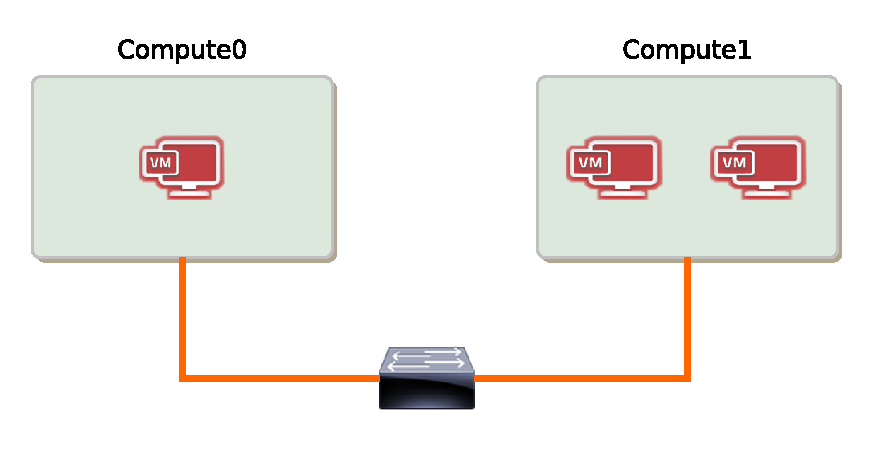
\includegraphics[width=0.8\textwidth]{diagrama.pdf}
    \caption{Esta es una figura que latex decide donde colocar (floating) en el documento.}
    \label{fig:diagrama}
    \end{figure}

    Latex decide dónde poner los elementos flotantes (figure o table)
    aunque usemos \verb#!htb# que significa: intenta poner el elemento
    aquí (h:here), al inicio de la página (t: top) o al final de la
    página (b: bottom). Sin embargo, a veces quedan demasiado lejos de
    donde son citados. Si esto ocurre puedes usar la orden
    \verb#\cleardoublepage# para que vacíe el buffer de elementos flotantes.

  \begin{tabular}{cc}
    Imagen 1 & Imagen 2 \\[2mm]
    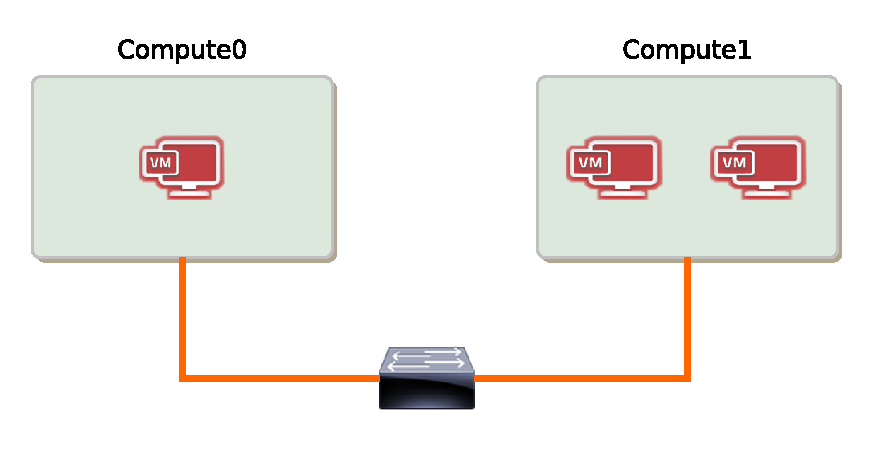
\includegraphics[width=0.4\textwidth]{diagrama.pdf} &  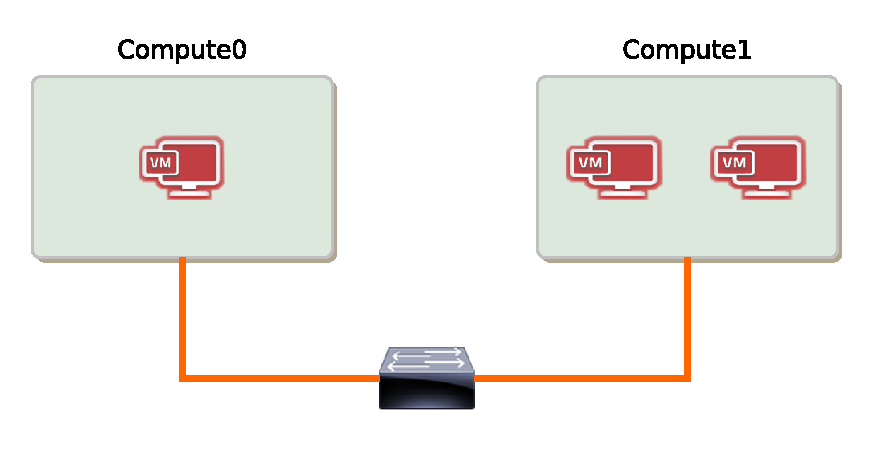
\includegraphics[width=0.4\textwidth]{diagrama.pdf}
  \end{tabular}

  La Tabla \ref{tbl:ejemplo} muestra un ejemplo.

\begin{table}[h!tb]
  \caption{Ejemplo de tabla \label{tbl:ejemplo}}
  \begin{tabular}{|l|c|}
    \hline
    Columna 1 & Columna 2 \\ \hline
    1 & 2 \\ \hline
  \end{tabular}
\end{table}


  \vspace*{1cm}
  Mientras que la Tabla \ref{tbl:centrada} muestra la misma tabla centrada. 

  \begin{table}[h!tb]
  \caption{Ejemplo de tabla centrada \label{tbl:centrada}}
  \begin{center}
    \begin{tabular}{|l|c|}
      \hline
      Columna 1 & Columna 2 \\ \hline
      1 & 2 \\ \hline
    \end{tabular}
  \end{center}
  
\end{table}

  Para generar el fichero PDF podemos usar los comandos que muestra el Listao \ref{lst:cmds}.

  \begin{lstlisting}[language=bash,caption={Comandos para generar PDF con pdflatex},label={lst:cmds}]
    pdflatex ejemplo-memoria.tex
    bibtex ejemplo-memoria
    pdflatex ejemplo-memoria.tex
\end{lstlisting}

  También se puede usar \texttt{latexmk} que automáticamente regenera la bibliografía, tal y como muestra el Listado \ref{lst:latexmk}.

  \begin{lstlisting}[language=bash,caption={Comandos para generar PDF con latexmk},label={lst:latexmk}]
    latexmk -pdf ejemplo-memoria.tex
\end{lstlisting}
